
\chapter{Exercise 2}
\label{cha:ugeopgave-2}

The purpose of this exercise is to understand the various method of setting up the virtual camera and to be able to adjust the parameters of the camera. We will get more acquainted with defining the matrices in the viewing pipeline and to concatenate them into the viewing matrix. Secondly, we will make different pictures of the scene using various projection method based on central projection (Front, X and 3-point perspective) and Orthographic parallel projection (Isometric, Dimetric, and Trimetric axonometric). Many of the principles will be demonstrated in OpenGL

\section{Part 1}
\label{sec:del-1:-isometri}

Vertex elements are considered in 2D space so their positions are represented cartesian coordinates.
On the other hand, in this exercise, vertex elements are in 3D space and their positions are represented in
homogenous coordinates, which are vec4.\\

In display function, we describe model-view properties of our vision (camera). In this exercise, it is defined with triplet of eye, at, up. LookAt() function, which takes an eye position, a position to look at, and an up vector,
all in object space coordinates computes the inverse camera transform according to its parameters
and multiplies it onto the current matrix stack.

\section{Part 2}
\label{sec:del-2:-viewing}

\begin{itemize}
  \item You can see resulting Figure \ref{fig:2-2}.
  \item Translation, rotation around Y axis, and Scaling
  \item Model matrix is similar with this:\\
      Translate(...)*RotateY(...)*Scale(..)\\
       Matrix multiplication is NOT a commutative operation so the order is \emph{important}.
\end{itemize}



\begin{figure}[hp]
\centering
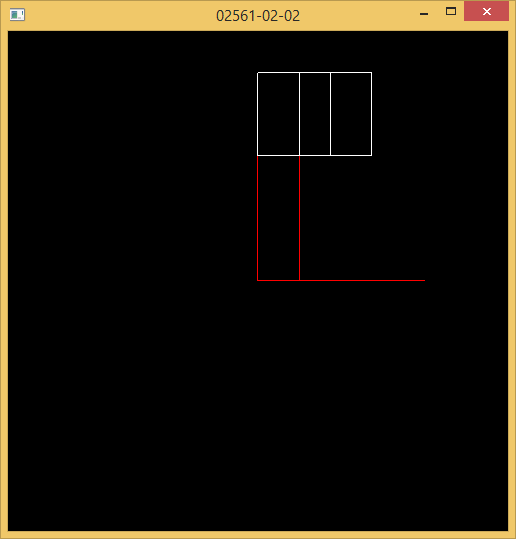
\includegraphics[width=8cm]{../Screenshots/ex-2/2.png}
\caption{After three transformations}
\label{fig:2-2}
\end{figure}

\section{Part 3}
\label{sec:del-3}

After following descriptions in exercise text, I reach the expected result. You can see front perspective screenshot in Figure \ref{fig:2-3}.
\begin{figure}[hp]
\centering
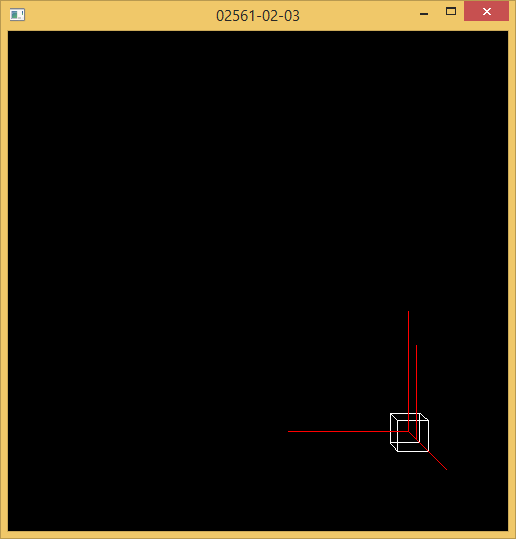
\includegraphics[width=8cm]{../Screenshots/ex-2/3.png}
\caption{Front Perspective}
\label{fig:2-3}
\end{figure}

\section{Part 4}
\label{sec:del-4}

I get the isometric view (see Figure \ref{fig:2-4}) by using this LookAt call as a View matrix :

\emph{LookAt(vec3(5,5,5), vec3(0,0,0), vec3(0,0,1))} \\
The idea is selecting the eye point on diagonal line of the cube. 

\begin{figure}[hp]
\centering
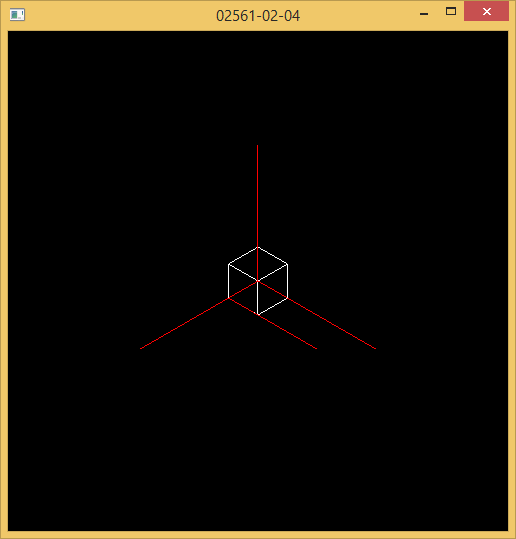
\includegraphics[width=8cm]{../Screenshots/ex-2/4.png}
\caption{Isometric View}
\label{fig:2-4}
\end{figure}


\section{Part 5}
\label{sec:del-5}

I make the necessary key assignments. 
\begin{itemize}
  \item Series of transformations for key 2 is \\
      \emph{RotateY(-atan(0.25)/DegreesToRadians)*Translate(vec3(+.5, -1, -6))}
  \item Corresponding lookAt function for key 4 is\\
      \emph{LookAt(vec3(4, 1, 1), vec3(4, 1, 1) + vec3(-sqrt(3), 0, 1), vec3(0,1,0))}
  \item The hardcoded matrix used in key 6 is\\
      \emph{mat4 ( 1,0,0,0,
				  0,1,0,0,
				  0,0,1,0,
				  1,-1,-9,1)}

To check the similarities of key couples 1-2, 3-4, and 5-6 please execute the program.
\end{itemize}

\section{Part 6}
\label{sec:del-6}

\begin{itemize}
  \item \emph{modelView=RotateX(atan(1.0/2)/DegreesToRadians)*
		Translate(0,-3,-6);}
  \item \emph{modelView=Translate(0,3,0)*RotateY(30)*Scale(2,2,2);}
\end{itemize}

%%% Local Variables:
%%% mode: latex
%%% TeX-master: "report_main"
%%% End:
